\documentclass{article}

\usepackage{tikz,tikz-qtree}
\usepackage{pgf,pgfsubpic}

\begin{document}

\fbox{%
\begin{pgfpicture}
\pgfnode{rectangle}{center}{Hello}{hellonode}{\pgfusepath{stroke}}
\begin{pgfsubpicture}
\pgfpathcircle{\pgfpointorigin}{4pt}\pgfusepath{stroke}
\pgfnode{rectangle}{center}{there}{therenode}{\pgfusepath{stroke}}
\end{pgfsubpicture}
\pgftransformshift{\pgfpoint{1in}{-1in}}
\pgftransformscale{2}
\pgftransformrotate{45}
\pgfpathcircle{\pgfpointorigin}{2pt}\pgfusepath{fill}
\pgfplacesubpicture

\pgfmoveto{\pgfpointanchor{hellonode}{south}}
\pgflineto{\pgfpointanchor{therenode}{north}}
\pgfusepath{stroke}

\end{pgfpicture}%
}

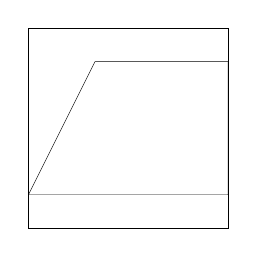
\begin{tikzpicture}
\begin{pgfscope}
\begin{pgfsubpicture}
\draw (-1in,0)--(2in,0)--(2in,2in)--(0,2in)--cycle;
\end{pgfsubpicture}
\pgffitsubpicture{\pgfpointorigin}{\pgfpoint{1in}{1in}}
\pgfplacesubpicture
\end{pgfscope}

\draw (0,0)--(1in,0)--(1in,1in)--(0,1in)--cycle;


\end{tikzpicture}




\end{document}
